\section{Additional Figures}\label{appFigures}

\textbf{
    In this section, we offer some additional examples of which our VSFs look at different times and considering different analysis approaches.
    In particular, we focus on the standard analyis (Sect.~\rc{!!! ref !!!}, Figs.~\rc{!!! ref !!!}), the density threshold-less scenario (Sect.~\rc{!!! ref !!!}, Figs.~\rc{!!! ref !!!}), and the impact analysis of different Jeans refinement levels (Sect.~\rc{!!! ref !!!}, Figs.~\rc{!!! ref !!!}).
}

\rc{continue?}
 	
\begin{figure*}
    \centering
    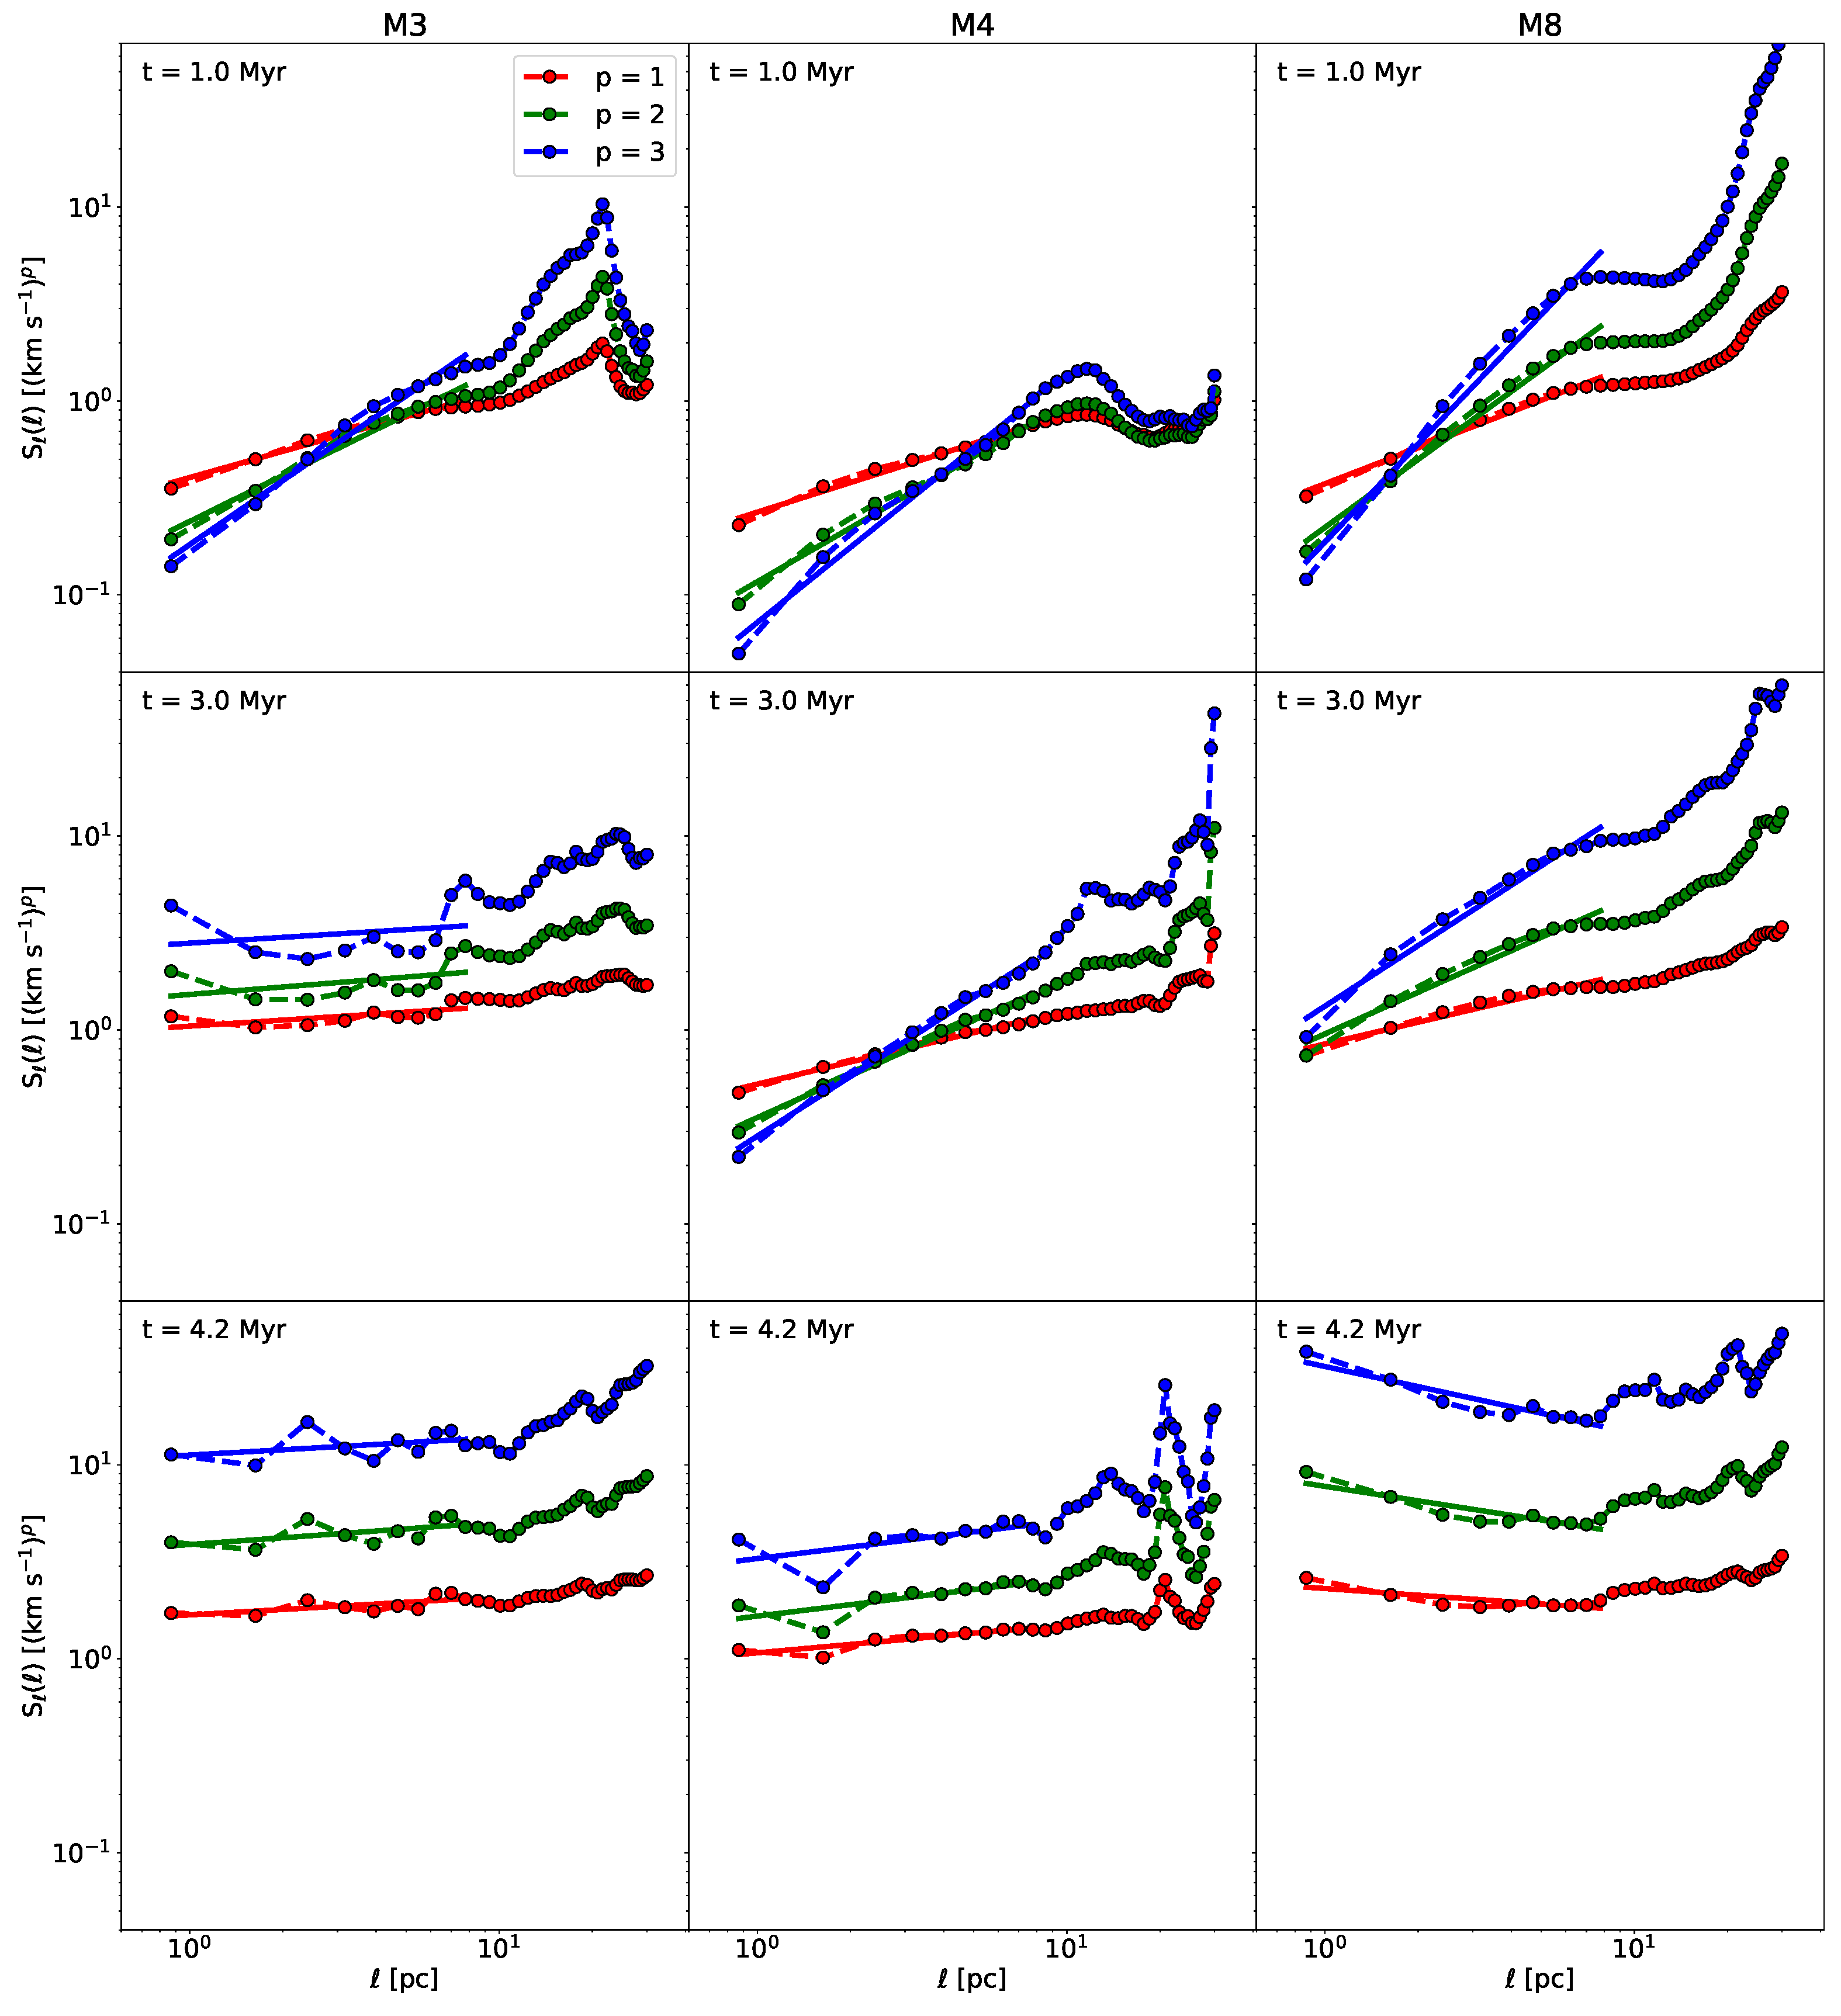
\includegraphics[width=\textwidth]{app_examples_wthres_s_l.pdf}
    \caption{
        The figures show additional examples of VSFs, based on data with density threshold, of (\textit{left} to \textit{right}) \texttt{M3}, \texttt{M4}, and \texttt{M8} as function of lag scale $\ell$ and order $p$. 
        The examples are given for three different time steps, namely (\textit{top} to \textit{bottom}) t~=~1.0~Myr, 3.0~Myr, and 4.2~Myr.
        The dots (connected by dashed lines) show the values computed from the simulations. 
        The solid lines represent the power-law relation fitted to the respective structure functions.
    }
    \label{pic:appFigures:examples_with_threshold_s_vs_l}
\end{figure*}
 	
 	
\begin{figure*}
    \centering
    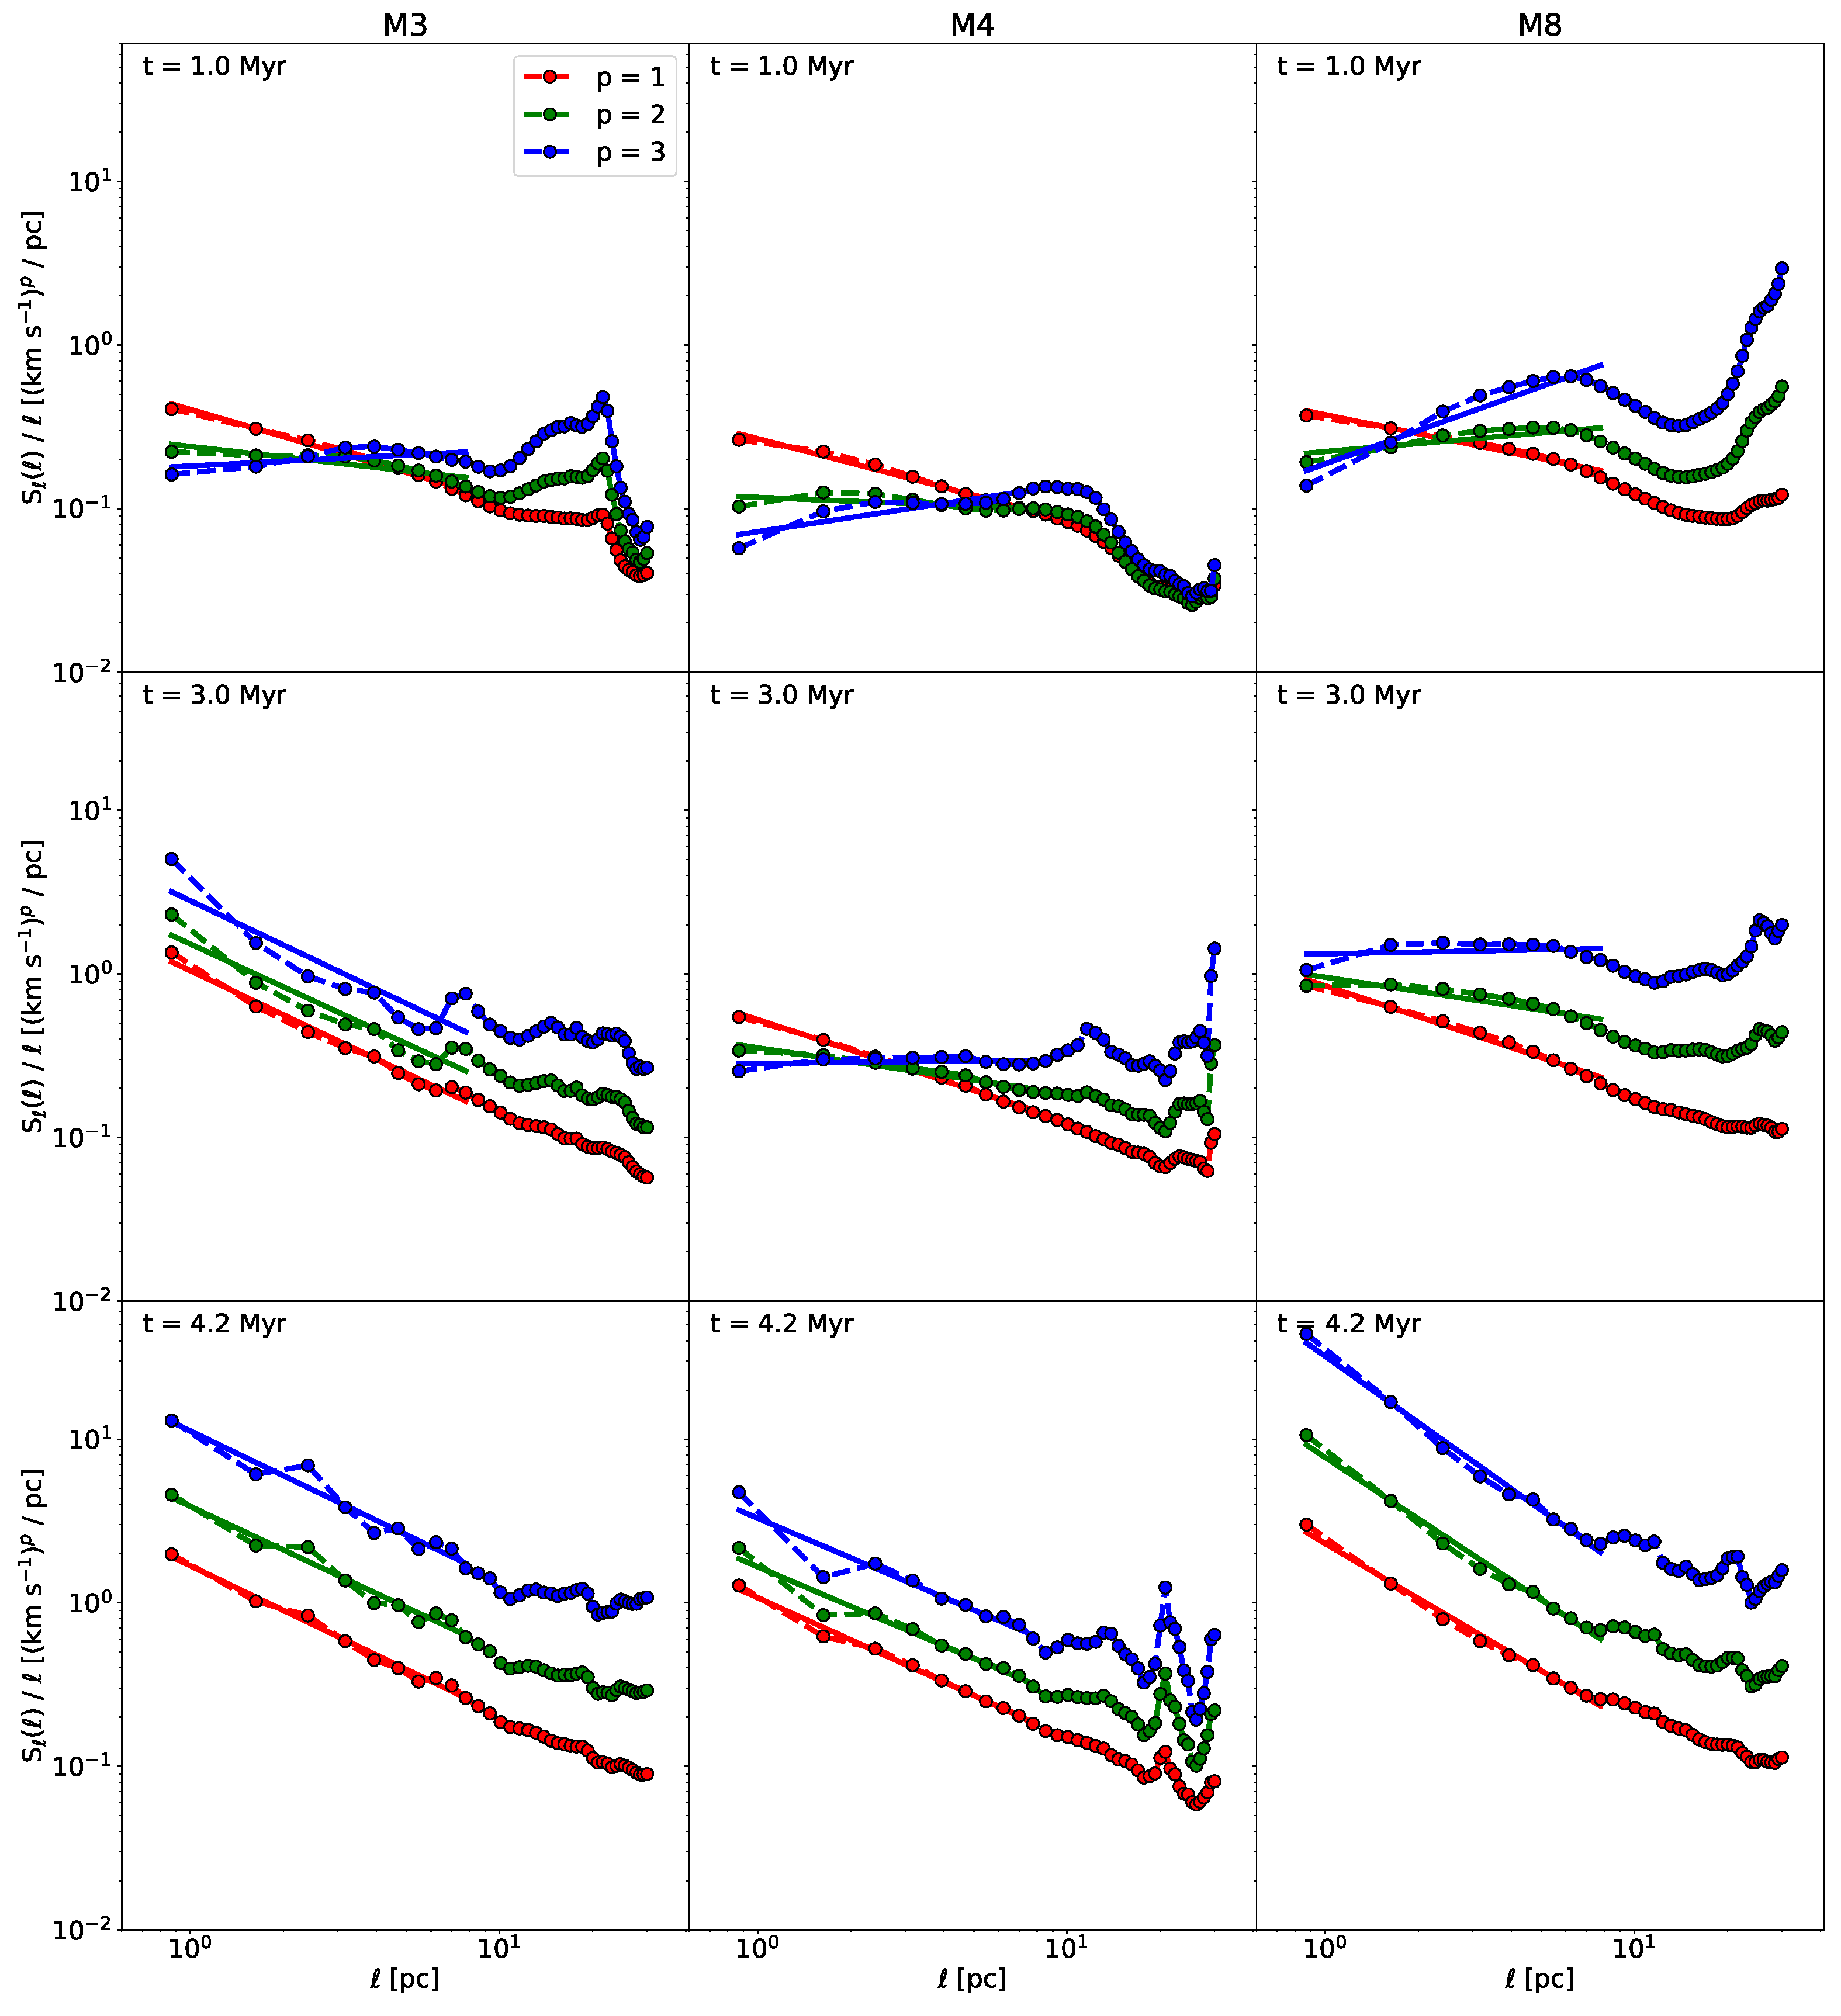
\includegraphics[width=\textwidth]{app_examples_wthres_sl_l.pdf}
    \caption{
        As Fig.~\ref{pic:appFigures:examples_with_threshold_s_vs_l}, but plotting the relation between S$_{\ell}$ / $\ell$ as function of lag scale $l$ and order $p$.
    }
    \label{pic:appFigures:examples_with_threshold_sl_vs_l}
\end{figure*}
 	
 	
\begin{figure*}
    \centering
    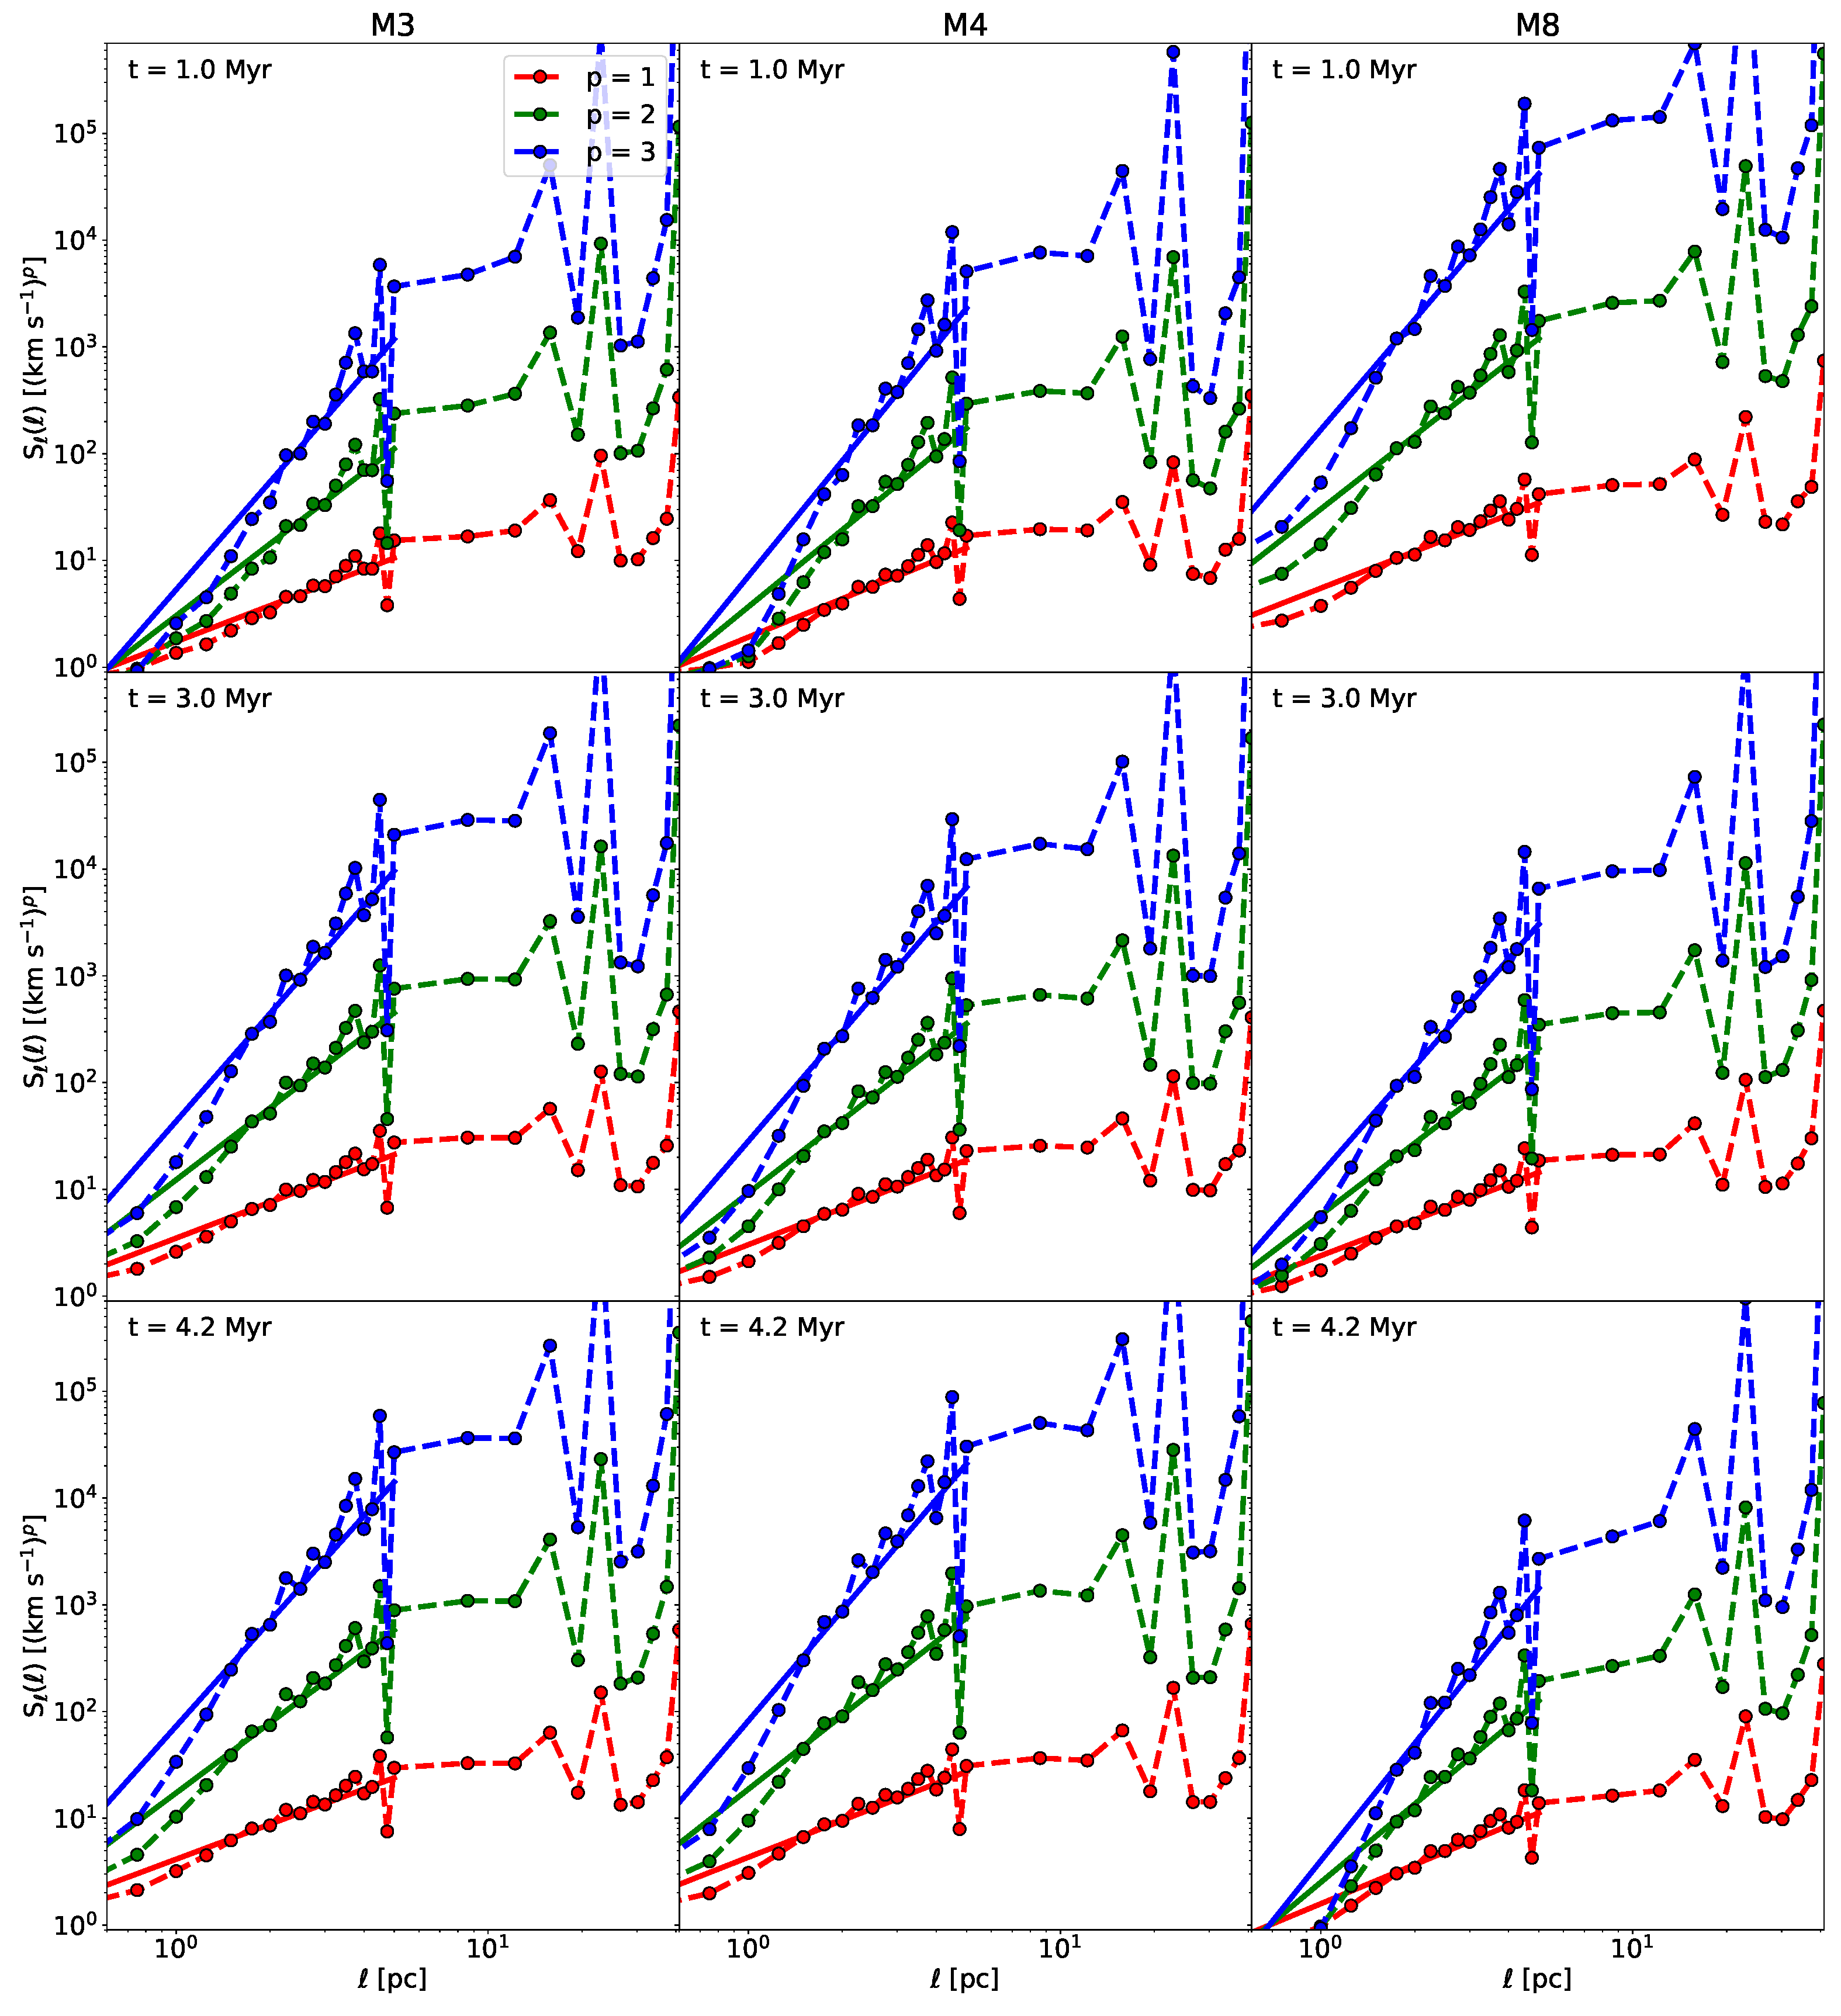
\includegraphics[width=\textwidth]{app_examples_woutthres_s_l.pdf}
    \caption{
        As Fig.~\ref{pic:appFigures:examples_with_threshold_s_vs_l}, but based on data without density threshold.
    }
    \label{pic:appFigures:examples_without_threshold_s_vs_l}
\end{figure*}
 	
 	
\begin{figure*}
    \centering
    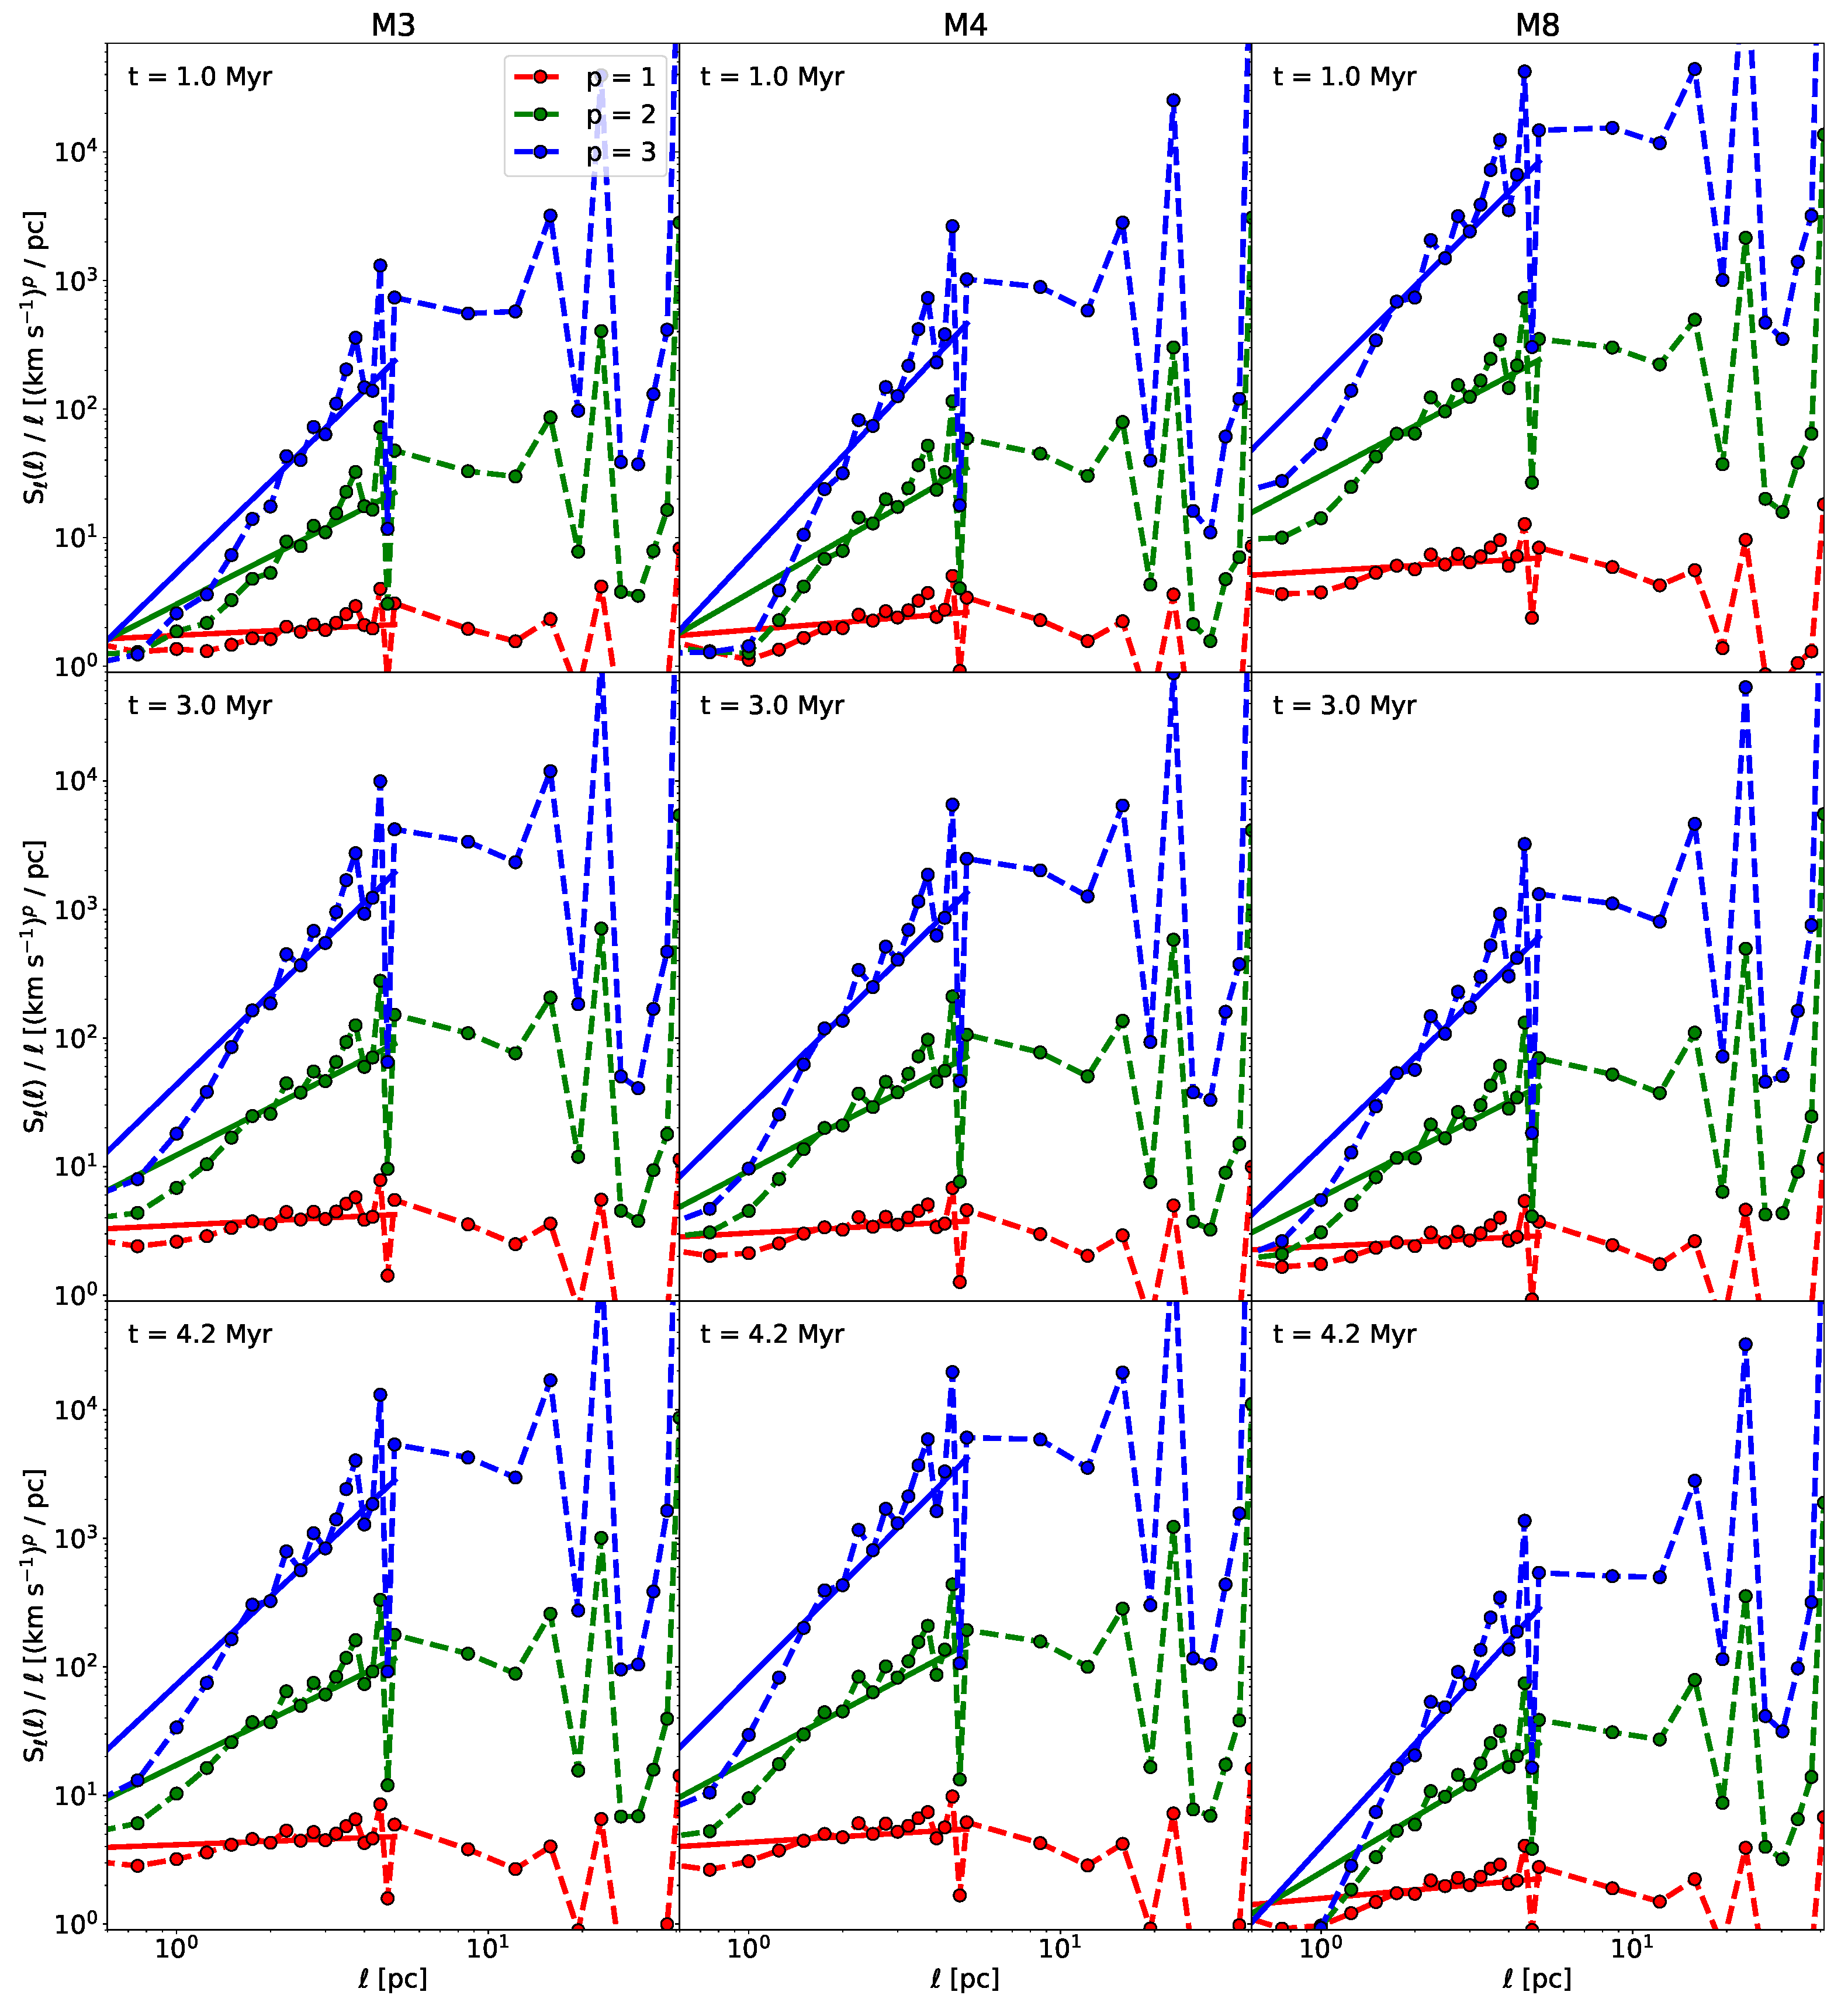
\includegraphics[width=\textwidth]{app_examples_woutthres_sl_l.pdf}
    \caption{
        As Fig.~\ref{pic:appFigures:examples_with_threshold_sl_vs_l}, but based on data without density threshold.
    }
    \label{pic:appFigures:examples_without_threshold_sl_vs_l}
\end{figure*}


 	
\begin{figure*}
    \centering
    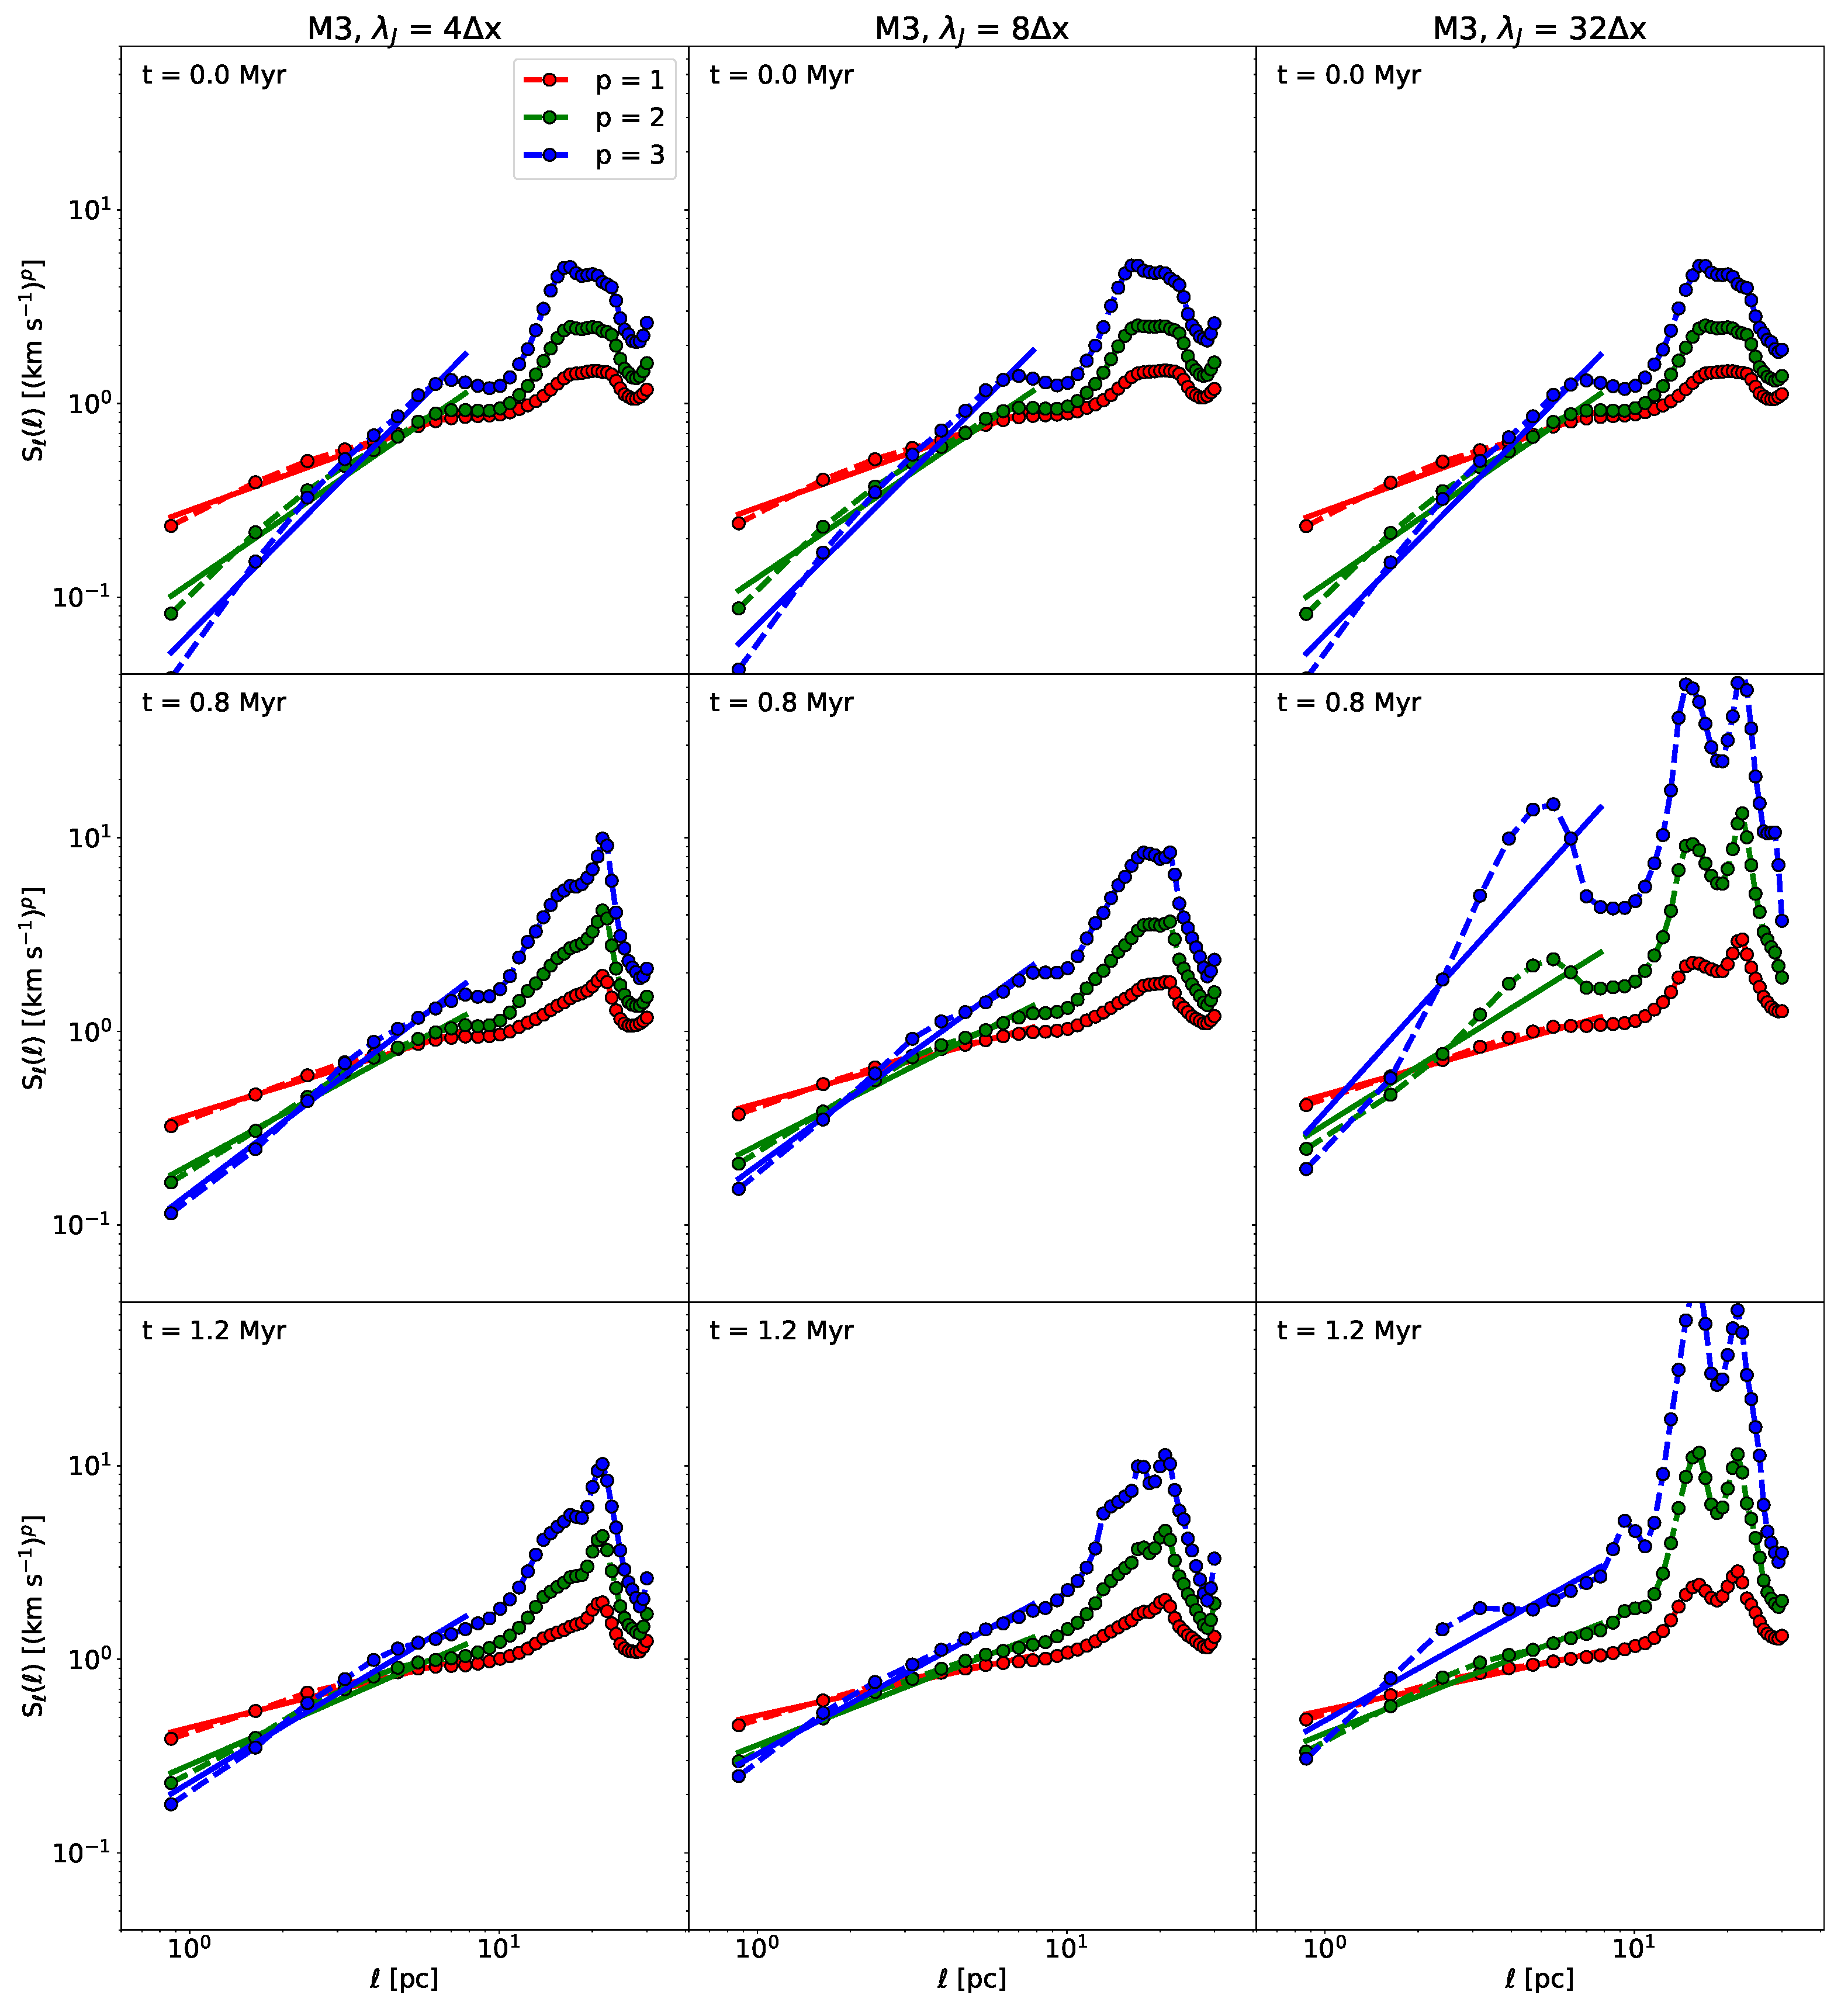
\includegraphics[width=\textwidth]{app_examples_jeans_s_l.pdf}
    \caption{
        The figures show additional examples of VSFs, based on data of \texttt{M3} with density threshold, at the different refinement levels (\textit{left} to \textit{right}) $\lambda$~=~4~$\Delta$x, $\lambda$~=~8~$\Delta$x, and $\lambda$~=~8~$\Delta$x as function of lag scale $\ell$ and order $p$. 
        The examples are given for three different time steps, namely (\textit{top} to \textit{bottom}) t~=~0.0~Myr, 0.8~Myr, and 1.2~Myr.
        The dots (connected by dashed lines) show the values computed from the simulations. 
        The solid lines represent the power-law relation fitted to the respective structure functions.
    }
    \label{pic:appFigures:examples_jeans_s_vs_l}
\end{figure*}


 	
\begin{figure*}
    \centering
    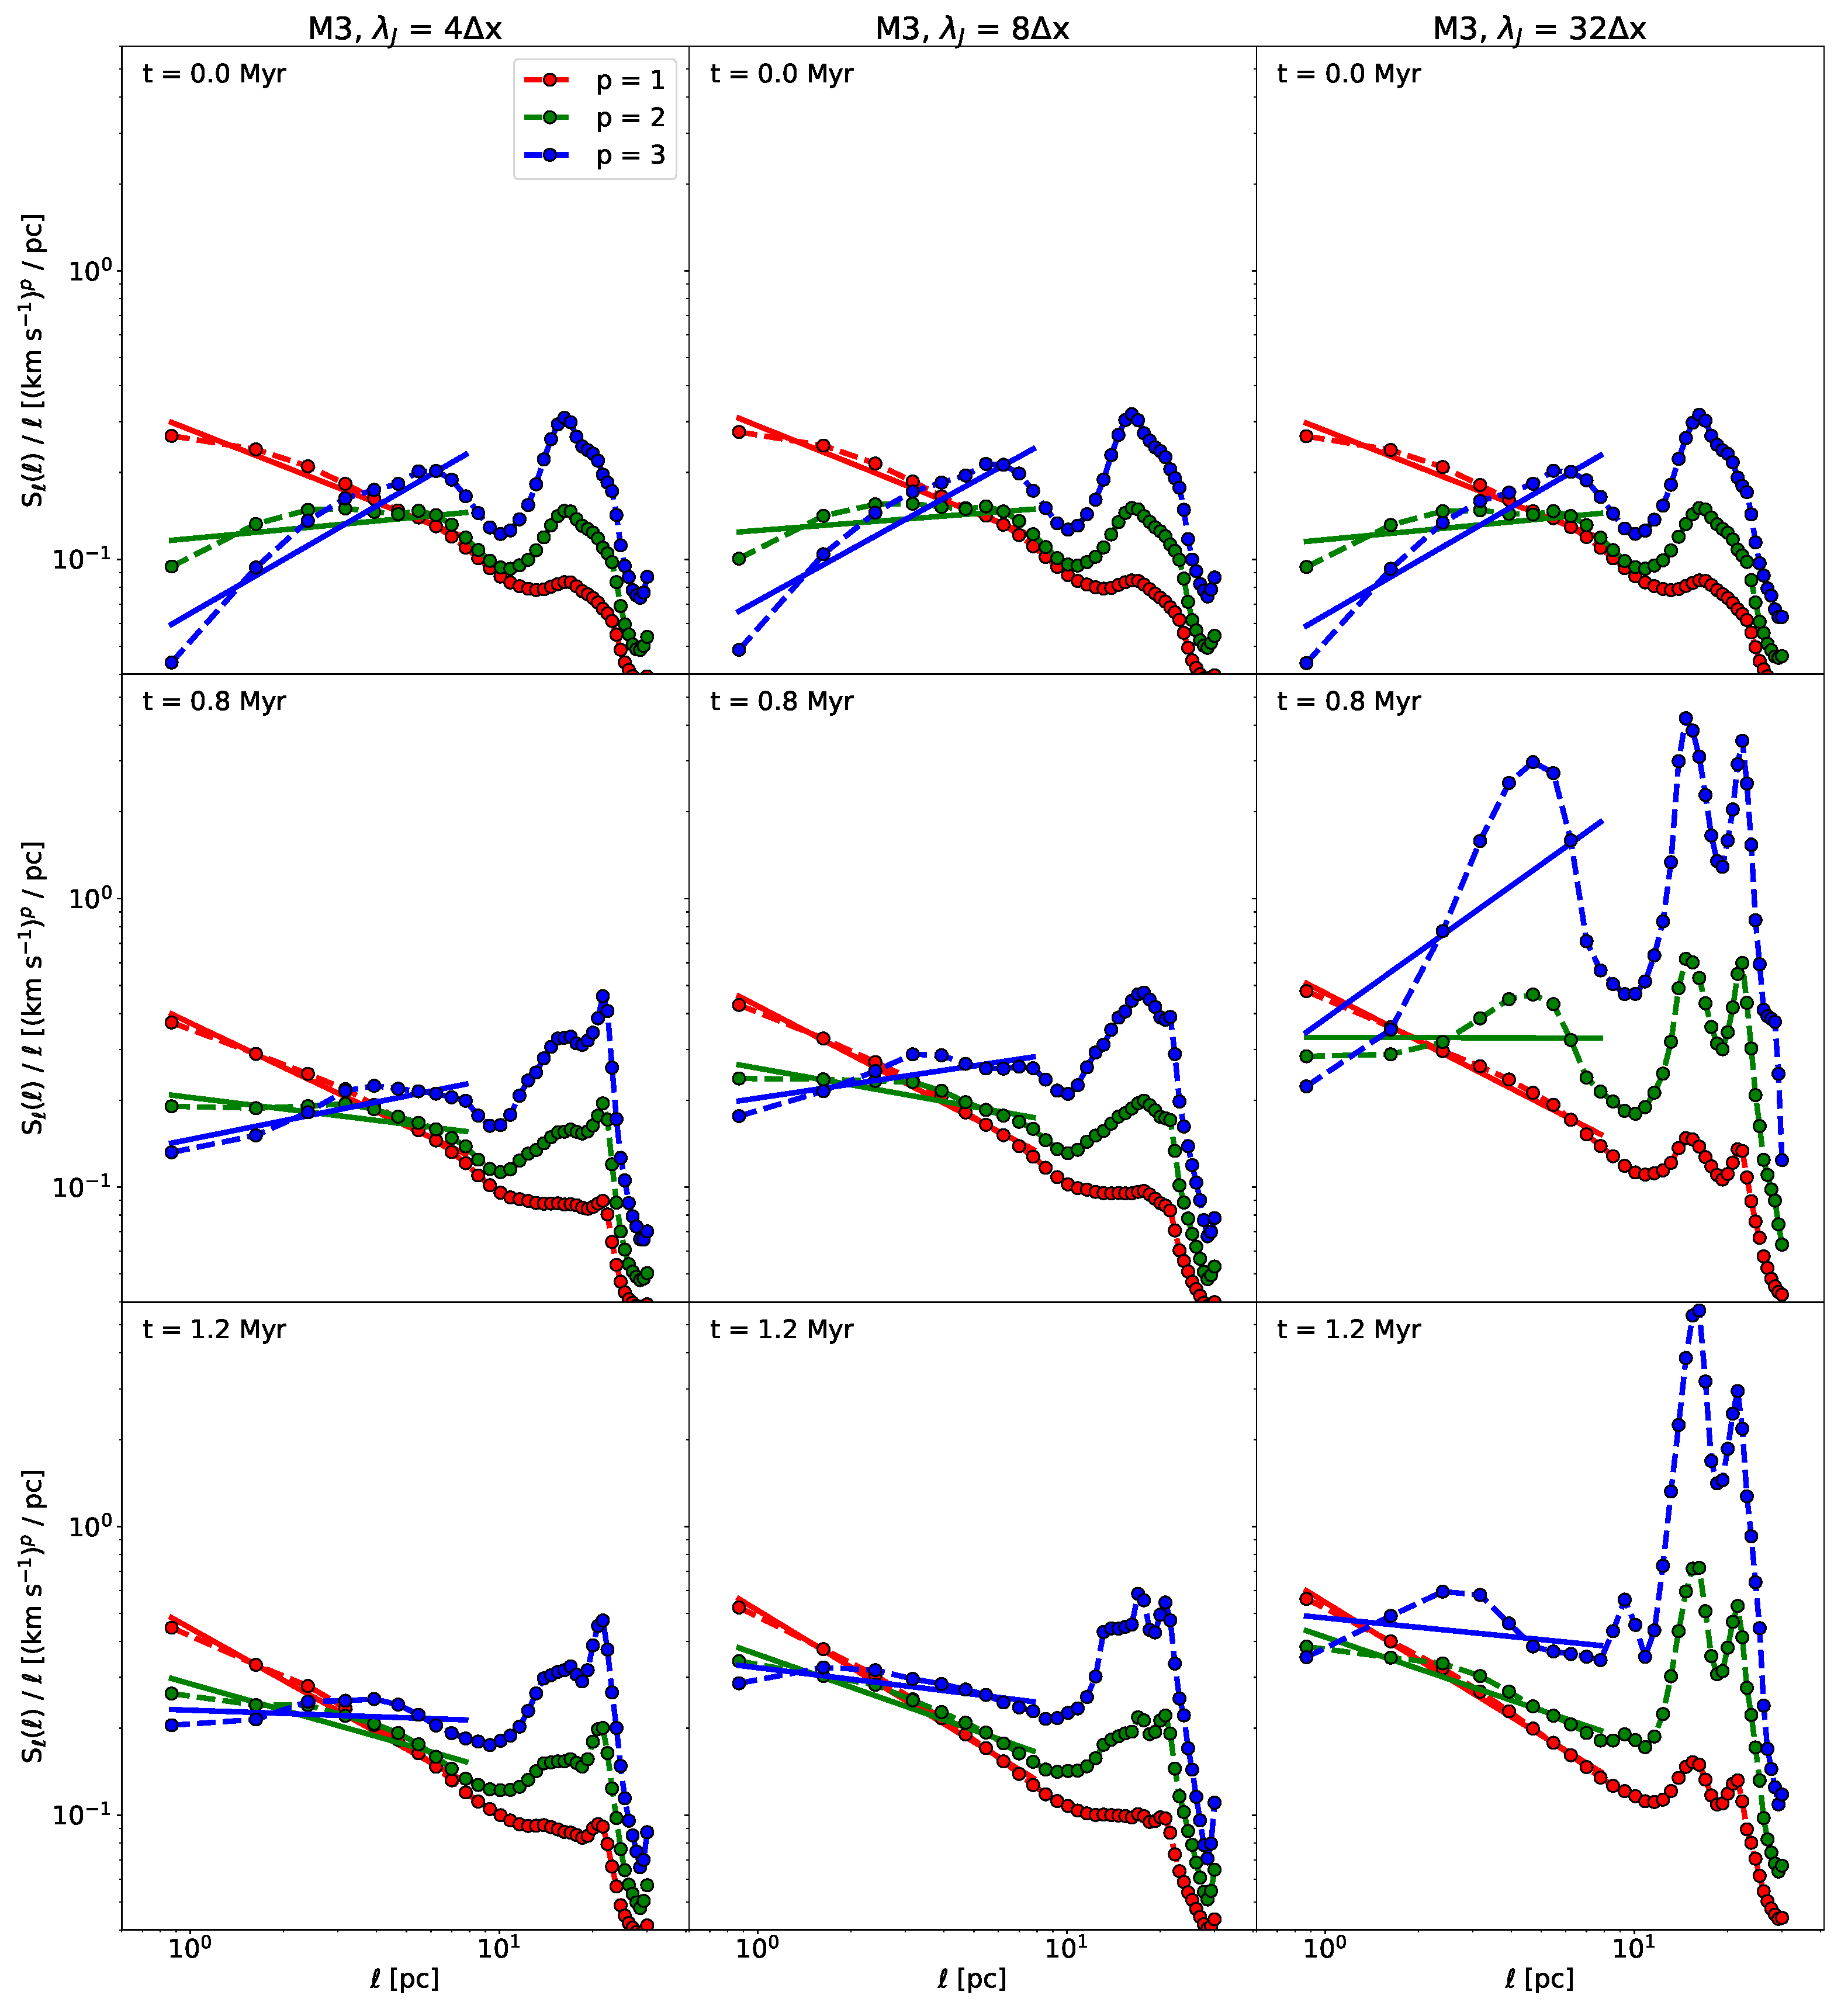
\includegraphics[width=\textwidth]{app_examples_jeans_sl_l.pdf}
    \caption{
        As Fig.~\ref{pic:appFigures:examples_jeans_s_vs_l}, but plotting the relation between S$_{\ell}$ / $\ell$ as function of lag scale $l$ and order $p$.
    }
    \label{pic:appFigures:examples_jeans_sl_vs_l}
\end{figure*}
